\chapter{反应的能量：燃烧与键能}\label{ch:g11:reaction-energy}

撕开暖手宝的封口，过一分钟，它就烫得不能长时间握在手里；
挤压冷敷袋，它就会使扭伤的脚踝变凉；一辆城市公交车整天烧氢气行驶，
尾气中只留下水蒸气。
化学变化不仅能把物质变成其他物质，还会释放能量或吸收能量。
这些能量从何而来，
一种燃料究竟能提供多少能量？

\begin{recall}
完全燃烧时，由碳和氢组成的燃料在氧气中燃烧，
生成二氧化碳和水
（见\cref{ch:g8:combustion-and-fuels}）。共价键是一对共用电子；路易斯结构
表示分子中的每一个化学键
（见\cref{ch:g10:lewis-and-shape}）。物质的量以摩尔计量
（见\cref{ch:g10:the-mole}）。
\end{recall}

\begin{omfigure}
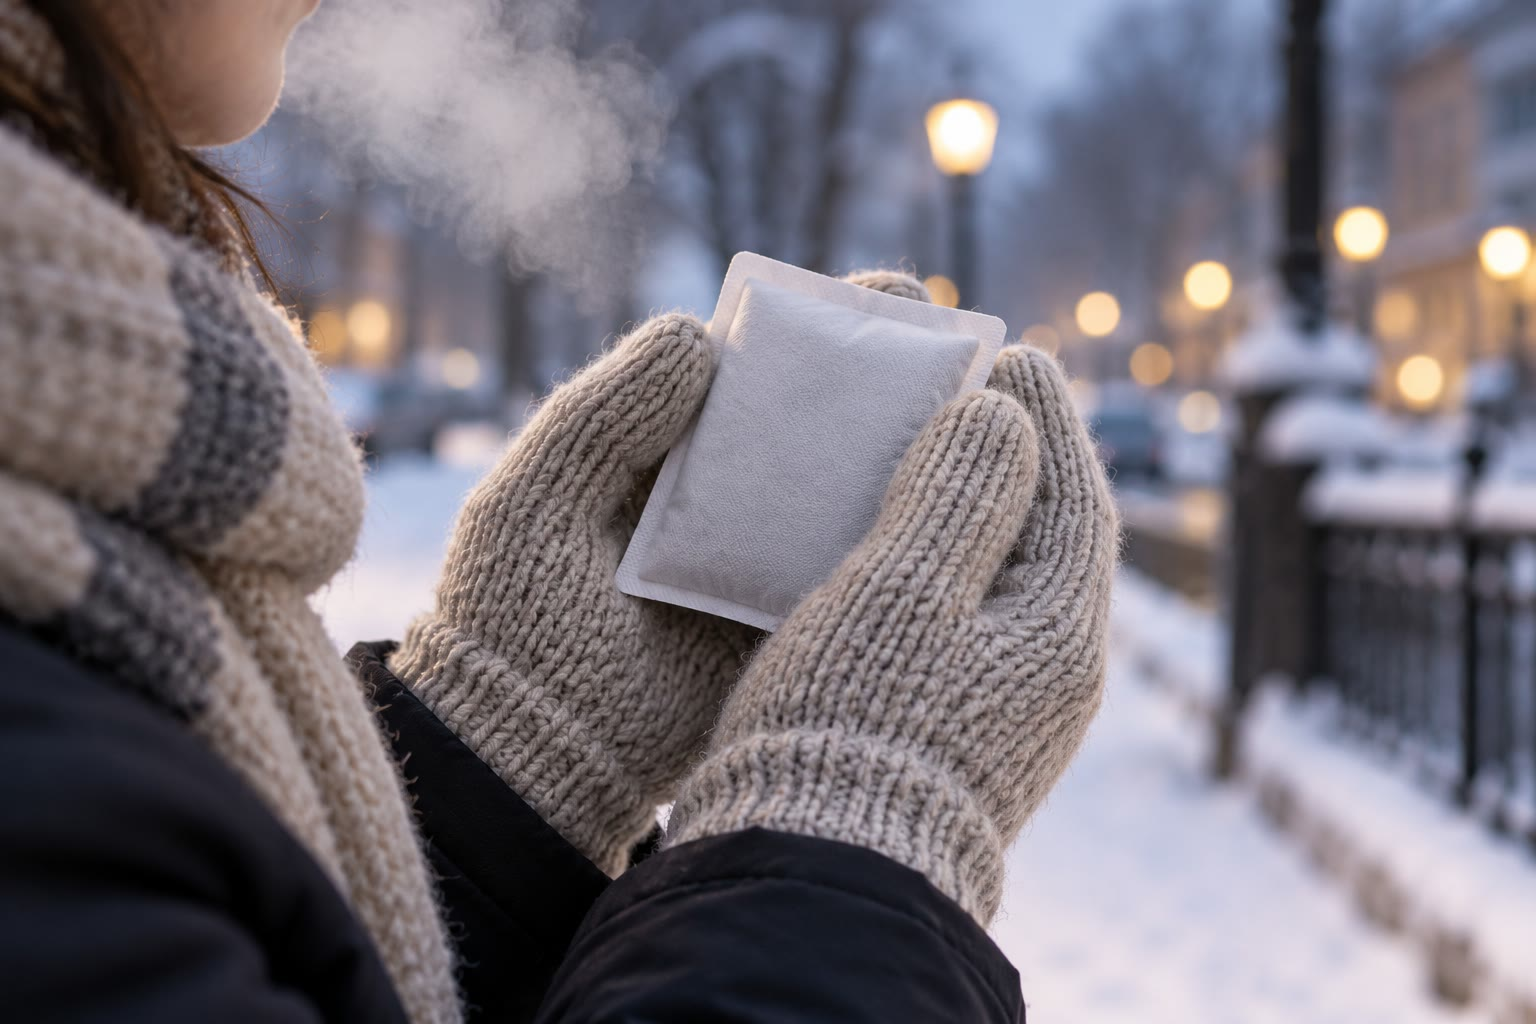
\includegraphics[width=0.45\linewidth]{images/book1/ai/g11-hand-warmers.jpg}

{\small 暖手宝：袋内的反应放出热量。}
\end{omfigure}

\section{放热过程与吸热过程}

\begin{definition}[放热、吸热]\label{def:g11:reaction-energy:exothermic}
若某一过程向外界释放能量（通常为热量），则称其为\emph{放热的}\index{放热的}，
此时外界温度升高。
若某一过程从外界吸收能量，则称其为\emph{吸热的}\index{吸热的}，
此时外界降温，或该过程需要加热才能
继续进行。
\end{definition}

\begin{example}[热与冷]\label{ex:g11:reaction-energy:packs}
燃烧是放热的，暖手宝中铁粉与空气中氧气的缓慢反应也是放热的。
用于冷敷袋的硝酸铵溶于水是吸热的；
石灰石分解为生石灰和二氧化碳也是吸热的，
这一分解只有在很高温的
窑中才能发生。
\end{example}

\begin{omfigure}
\begin{tikzpicture}[font=\small]
  \begin{scope}
    \draw[->] (0,0) -- (0,3.2) node[above] {能量};
    \draw[very thick, omDef] (0.5,2.5) -- (2.3,2.5) node[right, text=black] {反应物};
    \draw[very thick, omProp] (0.5,0.8) -- (2.3,0.8) node[right, text=black] {生成物};
    \draw[->, thick, omThm] (1.4,2.45) -- (1.4,0.85);
    \node[omThm, anchor=west, align=left] at (1.5,1.65) {能量 \\ 释放};
    \node[anchor=north] at (1.6,-0.15) {\textbf{放热}};
  \end{scope}
  \begin{scope}[xshift=6cm]
    \draw[->] (0,0) -- (0,3.2) node[above] {能量};
    \draw[very thick, omDef] (0.5,0.8) -- (2.3,0.8) node[right, text=black] {反应物};
    \draw[very thick, omProp] (0.5,2.5) -- (2.3,2.5) node[right, text=black] {生成物};
    \draw[->, thick, omDef] (1.4,0.85) -- (1.4,2.45);
    \node[omDef, anchor=west, align=left] at (1.5,1.65) {能量 \\ 吸收};
    \node[anchor=north] at (1.6,-0.15) {\textbf{吸热}};
  \end{scope}
\end{tikzpicture}

{\small 能量图。放热反应中，生成物所含能量比反应物少，
二者之差即为释放的能量；吸热反应中则相反，
生成物所含能量更多，须由外界提供。}
\end{omfigure}

\section{燃烧释放的能量}

\begin{definition}[摩尔燃烧能]\label{def:g11:reaction-energy:combustion-energy}
燃料的\emph{摩尔燃烧能}\index{摩尔燃烧能}记为 $E_c$，
即燃料完全燃烧一摩尔时所释放的能量，单位为 \si{kJ/mol}，
其中生成的水为液态。
\end{definition}

\begin{proposition}[$n$ 摩尔释放的能量]\label{prop:g11:reaction-energy:n-moles}
% ledger: dch:CH4
完全燃烧物质的量为 $n$ 的燃料时，释放的能量
为 $Q = n \times E_c$。对甲烷，$E_c = \qty{890.7}{kJ/mol}$，燃烧
\qty{1.00}{mol}（\qty{16.0}{g}）甲烷，约释放 \qty{891}{kJ} 能量。
\end{proposition}

\begin{proof}
每摩尔燃料燃烧释放 $E_c$；
则 $n$ 摩尔释放的能量为其 $n$ 倍。
\end{proof}

\begin{inthelab}[用酒精灯加热水]
% ledger: cp:water
先称量盛有乙醇的酒精灯，然后点燃它，给盛有
\qty{200}{g} 水的金属罐加热，罐中插有温度计。当水温升高
\qty{25}{\celsius} 时，熄灭火焰，再称量酒精灯，其质量已减少
\qty{1.50}{g} 的乙醇。水吸收的能量
可用物理学公式 $Q = m\, c\, \Delta\theta$ 计算，
其中 $c = \qty{4.18}{J/(g.\celsius)}$ 是水的比热容。
这一数值远小于乙醇所能释放的能量：大部分热量
用于加热空气、金属罐和酒精灯，还有部分乙醇
发生不完全燃烧。
\end{inthelab}

\begin{omfigure}
\begin{tikzpicture}[font=\small]
  % spirit burner
  \fill[black!8, draw=black!60] (-0.6,0) rectangle (0.6,0.7);
  \fill[cyan!15] (-0.55,0.05) rectangle (0.55,0.45);
  \fill[black!40] (-0.06,0.7) rectangle (0.06,0.95);
  \fill[orange!70!yellow] (0,0.95) .. controls (-0.25,1.25) and (-0.1,1.6) .. (0,1.85)
    .. controls (0.1,1.6) and (0.25,1.25) .. (0,0.95);
  \fill[yellow!40] (0,1.0) .. controls (-0.1,1.2) and (-0.05,1.4) .. (0,1.5)
    .. controls (0.05,1.4) and (0.1,1.2) .. (0,1.0);
  % tripod and can
  \draw[black!60, line width=1pt] (-1.1,0) -- (-0.9,2.1) (1.1,0) -- (0.9,2.1);
  \draw[black!60, line width=1.2pt] (-1.1,2.1) -- (1.1,2.1);
  \fill[black!15, draw=black!60] (-0.8,2.1) rectangle (0.8,3.7);
  \fill[omWater] (-0.75,2.15) rectangle (0.75,3.3);
  % thermometer
  \pic at (0.35,2.35) {thermometer};
  \draw[omProp, thick, <-] (0.6,0.35) -- (2.0,0.35) node[right, text=black]
    {酒精灯（乙醇）};
  \draw[omProp, thick, <-] (0.8,2.9) -- (2.0,2.9) node[right, text=black]
    {金属罐：\qty{200}{g} 水};
  \draw[omProp, thick, <-] (0.45,5.0) -- (2.0,5.0) node[right, text=black]
    {温度计};
\end{tikzpicture}

{\small 测量燃料提供的能量：酒精灯加热一个盛水的金属罐，
并测量水的温升。}
\end{omfigure}


\begin{example}[酒精灯的数值计算]\label{ex:g11:reaction-energy:burner}
% ledger: cp:water, dch:C2H5OH, aw:C, aw:H, aw:O
水吸收的热量为 $Q = 200 \times 4.18 \times 25 = \qty{2.09e4}{J}$，
即 \qty{20.9}{kJ}。燃烧的乙醇为 \qty{1.50}{g}，
其物质的量为 $1.50 / 46.0 = \qty{0.0326}{mol}$；若取 $E_c = \qty{1367.6}{kJ/mol}$，
则它可放出 $0.0326 \times 1367.6 = \qty{44.6}{kJ}$。
其中只有 $20.9 / 44.6 \approx \qty{47}{\percent}$ 传给了水。
\end{example}

\section{键能}

\begin{definition}[键能]\label{def:g11:reaction-energy:bond-energy}
共价键的\emph{键能}\index{键能}是指
断开一摩尔此类键所需的能量（分子和原子均处于
气态）。表中数值是对大量分子测得的
平均值，单位为 \si{kJ/mol}。
\end{definition}

\begin{omfigure}
\small
% ledger: be:H-H, be:C-H, be:N-H, be:O-H, be:H-Cl, be:C-C, be:CC-double, be:C-O, be:CO-double, be:NN-triple, be:OO-double, be:Cl-Cl
\begin{tabular}{lr@{\qquad}lr@{\qquad}lr}
\hline
 键 & \si{kJ/mol} & 键 & \si{kJ/mol} & 键 & \si{kJ/mol} \\
\hline
\ce{H-H} & 436 & \ce{C-C} & 345 & \ce{O=O} & 498 \\
\ce{C-H} & 415 & \ce{C=C} & 611 & \ce{N#N} & 946 \\
\ce{N-H} & 390 & \ce{C-O} & 350 & \ce{Cl-Cl} & 243 \\
\ce{O-H} & 464 & \ce{C=O} & 741 & \ce{H-Cl} & 432 \\
\hline
\end{tabular}\par\medskip

{\small 平均键能。断开化学键总是需要吸收能量；
形成化学键则放出等量的能量。}
\end{omfigure}

\begin{omfigure}
\begin{tikzpicture}[font=\small, x=1cm, y=0.0015cm]
  \draw[->] (0,-850) -- (0,2900) node[above] {能量 (\si{kJ})};
  \draw[very thick, black!60] (0.4,2656) -- (3.9,2656);
  \node[anchor=west] at (4.0,2656) {分立原子： \ce{C + 4H + 4O}};
  \draw[very thick, omDef] (0.4,0) -- (3.9,0);
  \node[anchor=west] at (4.0,0) {\ce{CH4 + 2O2}};
  \draw[very thick, omProp] (0.4,-682) -- (3.9,-682);
  \node[anchor=west] at (4.0,-682) {\ce{CO2 + 2H2O}};
  \draw[->, thick, omDef] (1.0,30) -- (1.0,2626);
  \node[omDef, anchor=west, align=left] at (1.05,1500) {断开 4 个 \ce{C-H}\\ 和 2 个 \ce{O=O}：\\ $+\qty{2656}{kJ}$};
  \draw[->, thick, omProp] (3.4,2626) -- (3.4,-652);
  \node[omProp, anchor=west, align=left] at (3.45,1200) {形成 2 个 \ce{C=O}\\ 和 4 个 \ce{O-H}：\\ $-\qty{3338}{kJ}$};
  \draw[<->, omThm, thick] (0.6,-10) -- (0.6,-672);
  \node[omThm, anchor=west] at (0.65,-341) {$E_r \approx \qty{-682}{kJ}$};
\end{tikzpicture}

{\small 甲烷的燃烧可看作两个假想步骤，计算时采用平均键能：
先断开所有键，再形成新的键。
估算值 \qty{-682}{kJ}（每摩尔甲烷）是放热的。}
\end{omfigure}

\begin{proposition}[反应能量的估算]\label{prop:g11:reaction-energy:estimate}
对于气体间的反应，吸收的能量 $E_r$（若能量被释放，则为负值）
近似为
\[
  E_r \approx \sum E(\text{断开的键}) - \sum E(\text{形成的键}) .
\]
若 $E_r < 0$，则形成新键所释放的能量多于
断开旧键所需的能量，即该反应为放热反应。
\end{proposition}

\begin{proof}
可将该反应想象为两步：先断开反应物的所有键，
这一过程耗费第一项的能量并得到分立的原子；随后生成物的键形成，
这一步放出第二项的能量。所得结果仅为
估计值，因为表中数值是对许多分子的平均。
\end{proof}

\begin{method}[由键能估算反应能量]\label{met:g11:reaction-energy:bonds}
\begin{enumerate}
  \item 写出配平的方程式，以及每种
        分子的路易斯结构。
  \item 统计反应物中断开的各类键与生成物中形成的各类键，
        并计入化学计量数。
  \item 将断开的键的能量相加，
        再减去形成的键的能量。
  \item 得出结论：结果为负则为放热反应。
\end{enumerate}
\end{method}

\begin{example}[氢气与氯气]\label{ex:g11:reaction-energy:hcl}
% ledger: be:H-H, be:Cl-Cl, be:H-Cl
对于 \ce{H2 + Cl2 -> 2HCl}：断开一个 \ce{H-H} 和一个 \ce{Cl-Cl}，
$436 + 243 = \qty{679}{kJ}$；形成两个 \ce{H-Cl}，$2 \times 432 =
\qty{864}{kJ}$。因此 $E_r \approx 679 - 864 = \qty{-185}{kJ}$，即每摩尔
反应是放热的。
\end{example}


\begin{remark}[估算与测量]\label{rem:g11:reaction-energy:compare}
% ledger: dch:CH4
燃烧一摩尔甲烷实际放出的能量为
\qty{890.7}{kJ}，大于估算值。原因有三：二氧化碳中的 \ce{C=O}
键比表中平均的 \ce{C=O} 键更强；
实测值对应液态水，水蒸气液化会放出更多能量；
平均键能只是平均值。键能法只能给出
符号和数量级，
而非精确值。
\end{remark}

\section{燃料比较}

\begin{omfigure}
\begin{tikzpicture}
\begin{axis}[xbar, width=0.78\linewidth, height=5.4cm, xmin=0, xmax=160,
    xlabel={每千克燃料燃烧放出的能量（\si{MJ/kg}）},
    symbolic y coords={ethanol, octane, propane, methane, hydrogen},
    ytick=data, yticklabels={乙醇, 辛烷, 丙烷, 甲烷, 氢气}, bar width=10pt, nodes near coords,
    nodes near coords style={font=\footnotesize, /pgf/number format/fixed,
      /pgf/number format/precision=1, /pgf/number format/fixed zerofill},
    tick label style={font=\small}, label style={font=\small},
    axis lines*=left, xmajorgrids, grid style={gray!20}, enlarge y limits=0.15]
  % ledger: dch:C2H5OH, dfh:C8H18, dfh:CO2, dfh:H2O-l, dch:C3H8, dch:CH4 (per kg with the book's molar masses)
  \addplot[fill=omProp!55, draw=omProp] coordinates {(29.7,ethanol) (48.0,octane)
    (50.4,propane) (55.7,methane) (142.9,hydrogen)};
\end{axis}
\end{tikzpicture}

{\small 下列五种燃料各一千克完全燃烧时放出的能量
（生成的水为液态）。氢气每千克放出的能量远多于其他燃料；
乙醇中已含氧，相当于已经部分“燃烧”过，
放出的能量最少。}
\end{omfigure}

\begin{example}[每兆焦耳的二氧化碳]\label{ex:g11:reaction-energy:co2}
% ledger: dch:CH4, dch:C2H5OH
燃烧一摩尔甲烷放出 \qty{890.7}{kJ} 的能量，同时生成一摩尔
二氧化碳，质量为 \qty{44.0}{g}。若取一兆焦耳，即 \qty{1000}{kJ}，
则所生成的二氧化碳质量为 $44.0 \times 1000 / 890.7 = \qty{49.4}{g}$。
乙醇燃烧时，每放出 \qty{1367.6}{kJ} 的能量便生成两摩尔二氧化碳，
因此每兆焦耳产生的二氧化碳为 $88.0 \times 1000 / 1367.6 = \qty{64.3}{g}$。氢气
不产生二氧化碳，其唯一产物是水。
\end{example}

\begin{omfigure}
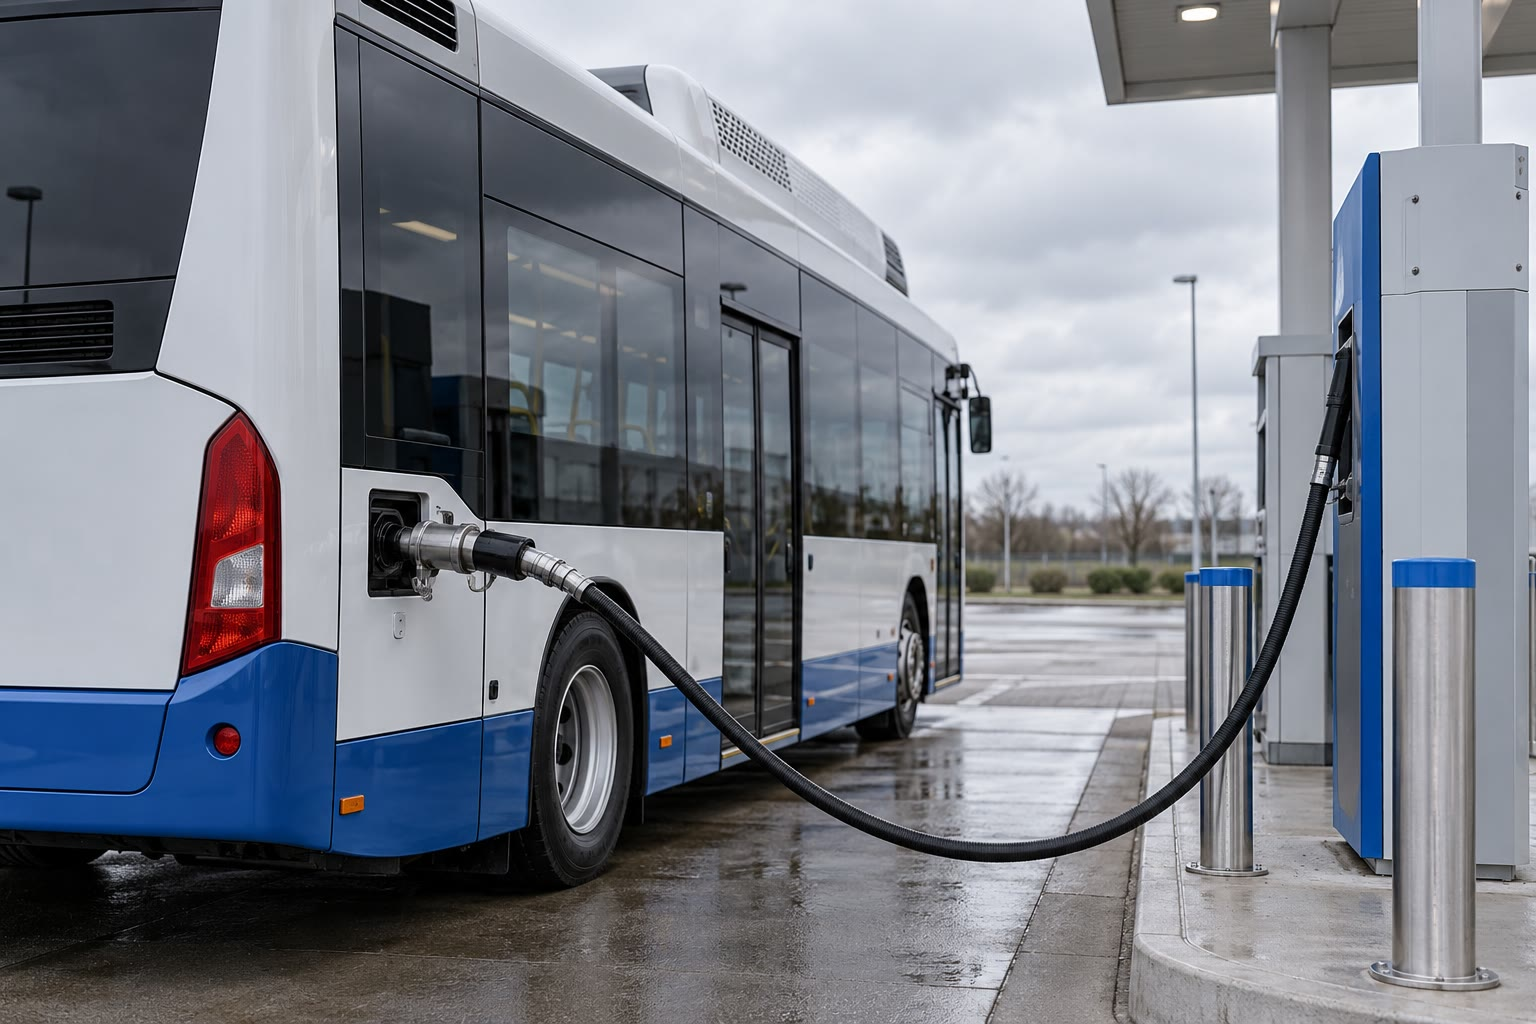
\includegraphics[width=0.5\linewidth]{images/book1/ai/g11-hydrogen-bus.jpg}

{\small 氢气加注站内的一辆公交车：其燃料燃烧后只生成水。}
\end{omfigure}

\begin{safety}{\ghs[0.82cm]{GHS02}\ghs[0.82cm]{GHS07}}
% ledger: ghs:ethanol
乙醇极易燃，并对眼睛有刺激性。酒精灯
应在远离明火处加注，热时不得补充，并由教师
在耐热垫上使用。
\end{safety}

\section{练习}


\begin{exercise}[$\star$]\label{exo:g11:reaction-energy:1}
判断下列过程是放热还是吸热：木材燃烧；冰熔化；
挤压冷敷袋；暖手宝发热；
绿叶在阳光下制造糖？
\end{exercise}

\begin{exercise}[$\star$]\label{exo:g11:reaction-energy:2}
% ledger: dch:CH4
求完全燃烧 \qty{3.0}{mol} 甲烷
放出的能量。
\end{exercise}

\begin{exercise}[$\star$]\label{exo:g11:reaction-energy:3}
在放热反应的能量图上，反应物与生成物中
哪一方所含能量更多？这部分能量差去了哪里？
\end{exercise}

\begin{exercise}[$\star$]\label{exo:g11:reaction-energy:4}
% ledger: dch:C2H5OH
求完全燃烧 \qty{100}{g} 乙醇
所放出的能量。
\end{exercise}

\begin{exercise}[$\star$]\label{exo:g11:reaction-energy:5}
什么是键能？为什么断开化学键总需要吸收能量？
\end{exercise}

\begin{exercise}[$\star\star$]\label{exo:g11:reaction-energy:6}
利用键能估算下列反应的能量，
\ce{2H2 + O2 -> 2H2O}，各物质均为气体。该反应是否放热？
\end{exercise}

\begin{exercise}[$\star\star$]\label{exo:g11:reaction-energy:7}
利用键能估算乙醇燃烧的能量，\ce{C2H5OH + 3O2 ->
2CO2 + 3H2O}（先画出乙醇的路易斯结构），
并与实测值 \qty{1367.6}{kJ/mol} 比较。
\end{exercise}

\begin{exercise}[$\star\star$]\label{exo:g11:reaction-energy:8}
% ledger: dch:C3H8, dch:CH4
计算每千克丙烷（\qty{2219.2}{kJ/mol}）
和甲烷放出的能量，并与条形图比较。
\end{exercise}

\begin{exercise}[$\star\star$]\label{exo:g11:reaction-energy:9}
% ledger: cp:water, dch:CH4
用燃气灶将 \qty{1.50}{L} 水（\qty{1500}{g}）
从 \qty{15}{\celsius} 加热到 \qty{100}{\celsius}。求水吸收的能量。
若这些能量全部传给水，需燃烧甲烷的质量为多少？
若只有一半能量传给水，质量又为多少？
\end{exercise}

\begin{exercise}[$\star\star$]\label{exo:g11:reaction-energy:10}
利用条形图，将各燃料按每千克放出的能量排序。
需要多少质量的氢气，才能放出与 \qty{1.0}{kg} 辛烷相同的能量？
\end{exercise}

\begin{exercise}[$\star\star$]\label{exo:g11:reaction-energy:11}
估算 \ce{N2 + 3H2 -> 2NH3} 的能量，各物质均为气体。
该反应是放热还是吸热？
\end{exercise}

\begin{exercise}[$\star\star\star$]\label{exo:g11:reaction-energy:12}
% ledger: cp:water, dch:C2H5OH
在一次酒精灯加热实验中，\qty{250}{g} 的水升高 
\qty{20}{\celsius}，同时燃烧了 \qty{1.20}{g} 乙醇。求水所吸收的
能量、乙醇可能放出的能量，以及加热的效率。
列举三个造成能量损失的原因。
\end{exercise}

\begin{exercise}[$\star\star\star$]\label{exo:g11:reaction-energy:13}
% ledger: dfh:C8H18, dfh:CO2, dfh:H2O-l, dch:C3H8
辛烷的摩尔燃烧能为 \qty{5470}{kJ/mol}，丙烷为 \qty{2219.2}{kJ/mol}。
写出它们的燃烧方程式，并计算各自每兆焦能量所放出的
二氧化碳质量。与甲烷比较，甲烷为 \qty{49.4}{g}。
\end{exercise}

\begin{exercise}[$\star\star\star$]\label{exo:g11:reaction-energy:14}
对甲烷和乙醇而言，
键能估算值均小于实测放出的能量。给出
原因，并说明为何该估算仍然有用。
\end{exercise}

\begin{exercise}[$\star\star\star$]\label{exo:g11:reaction-energy:15}
估算反应 \ce{2H2O -> 2H2 + O2} 的能量，各物质均为气体。
为什么由水制取氢气必须提供能量（例如电能）？
试解释为什么说氢气是一种\emph{储存}能量的方式，
而不是能量来源。
\end{exercise}

\section{问题：城市公交车应使用哪种燃料？}

\begin{problem}[{周末问题——甲烷、乙醇、辛烷与氢气：
哪一种每千克放出的能量最多，以及每兆焦
放出多少二氧化碳？}]
\label{pb:g11:reaction-energy:1}
% ledger: dch:CH4, dch:C2H5OH, dfh:C8H18, dfh:CO2, dfh:H2O-l, be:C-H, be:OO-double, be:CO-double, be:O-H
某城市比较了四种公交车用燃料：甲烷（天然气）、乙醇、
辛烷（代表汽油）和氢气。1 摩尔物质完全燃烧所放出的能量分别为：甲烷
\qty{890.7}{kJ}，乙醇 \qty{1367.6}{kJ}，辛烷
\qty{5470}{kJ}，氢气 \qty{285.8}{kJ}，
其中生成的水为液态。

\medskip
\noindent\textbf{第一部分——燃烧方程式。}
\begin{enumerate}
  \item 写出甲烷完全燃烧的方程式。
  \item 写出乙醇（\ce{C2H6O}）完全燃烧的方程式。
  \item 写出辛烷（\ce{C8H18}）完全燃烧的方程式。
  \item 写出氢气完全燃烧的方程式。
  \item 哪一种燃料不放出二氧化碳？
\end{enumerate}

\medskip
\noindent\textbf{第二部分——每千克能量。}
\begin{enumerate}[resume]
  \item 计算四种燃料的摩尔质量。
  \item 计算每种燃料每千克放出的
        能量（以 \si{MJ/kg} 为单位）。
  \item 对燃料进行排序。
  \item 氢气远胜其他燃料，但它仍难以用于
        公交车？（想一想它在室温下的状态。）
\end{enumerate}

\medskip
\noindent\textbf{第三部分——利用键能估算。}
\begin{enumerate}[resume]
  \item 画出甲烷燃烧所涉及分子的
        路易斯结构，并数出断裂和形成的化学键数目。
  \item 计算断开化学键所需的能量。
  \item 计算形成新化学键所放出的能量。
  \item 由此推算 $E_r$ 的估算值，并与
        实测值比较，相对差值是多少？
  \item 给出造成该差值的两个原因。
\end{enumerate}

\medskip
\noindent\textbf{第四部分——每兆焦的二氧化碳排放。}
\begin{enumerate}[resume]
  \item 要放出 \qty{1}{MJ} 的能量，需要燃烧多少物质的量的甲烷？
  \item 此时放出的二氧化碳质量是多少？
  \item 对乙醇和辛烷，重复上述问题。
  \item 在放出相同能量时，哪种含碳燃料放出的
        二氧化碳最少？为什么？（比较碳原子和氢原子的数目。）
  \item 氢气燃烧时不放出二氧化碳，但其对气候的真正益处
        取决于什么？
  \item 给出最终答案：每兆焦甲烷放出的
        二氧化碳质量是多少？
\end{enumerate}
\end{problem}
